

\documentclass{beamer}
 
\usepackage[utf8]{inputenc}
\usepackage{pgfpages}
\usepackage{array}

\setbeameroption{hide notes}
 
%Information to be included in the title page:
\title[Evolving Mean-Update Selection Methods for CMA-ES]
{Evolving Mean-Update Selection Methods for CMA-ES}
 
\author[Richter, Samuel \& Tauritz, Daniel] % (optional, for multiple authors)
{Samuel Richter (snr359@mst.edu) \\Daniel Tauritz (dtauritz@acm.org)}
 
\institute % (optional)
{
  Natural Computation Laboratory\\
  Department of Computer Science\\
  Missouri University of Science and Technology\\
  Rolla, Missouri 65409
}
 
\date{ECADA @ GECCO, July 2019}
 
\usetheme{Copenhagen}
 
\begin{document}
 
	\frame{\titlepage}
	
	\begin{frame}
		\frametitle{Introduction}
		
		\begin{itemize}
			 \item<1-|alert@1> Covariance-Matrix Adaptation Evolution Strategies (CMA-ES) use a sample-update cycle to optimize functions
			 \item<2-|alert@2> CMA-ES keep several state variables, including search space mean, evolution path, and covariance matrix
			 \item<3-|alert@3> Search space mean is updated every generation using sampled points
		\end{itemize}
	\end{frame}

	\begin{frame}
		\frametitle{Overview}

		\begin{itemize}
			\item<1-|alert@1> We wish to tune CMA-ES to a particular problem class
			\item<2-|alert@2> We do this by tuning the mean-update method
			\item<3-|alert@3> We evolve a new method of selecting the points used to update the mean
		\end{itemize}
	\end{frame}
	
	\begin{frame}
		\frametitle{Objective}
		\begin{itemize}
			 \item<1-> Objective: use a Hyper-Heuristic to generate a new mean-update selection function for CMA-ES to tune it to a problem class
			 \item<2-|alert@2> Step 1: define a representation for selection functions to form a search space
			 \item<3-|alert@3> Step 2: explore this space and determine the quality of the selection functions to find the best one
		\end{itemize}	
	\end{frame}	
			
	\begin{frame}
		\frametitle{Selection Function Representation}
		
		\begin{itemize}
			 \item<1-|alert@1> We use a two-part structure to represent a selection function
			 \item<2-|alert@2> The first part is a GP-Tree encoding a real-valued function of each point's fitness, fitness ranking, and other metrics, returning a "desirability" score for each point
			 \item<3-|alert@3> The second part is a final selection step that selects points based on their desirability scores
			 
		
		\end{itemize}
	\end{frame}
	
	\begin{frame}
		\frametitle{Representation}
		A selection function is represented by a mathematical function (encoded in a parse tree) and a selection method.
		\begin{center}
			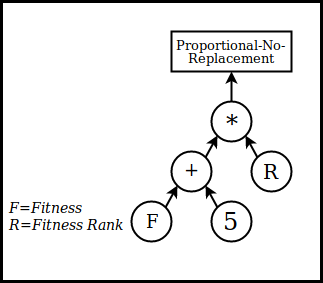
\includegraphics[height=0.6\textheight]{example_eppsea_nolabel}
		\end{center}
	\end{frame}
	
	\begin{frame}
		\frametitle{Meta-EA}
		
		\begin{itemize}
			 \item<1-|alert@1> We use a meta-EA to search through the space of possible mean-update selection functions
			 \item<2-|alert@2> Koza-style GP is used to evolve the trees, with an extra gene encoding the final selection step and any parameters to it	 
			 \item<3-|alert@3> Each run of the meta-EA targets one of the 24 noiseless test functions in the Comparing Continuous Optimizers function set
 			 \item<4-|alert@4> Dimensions of 2, 3, 5, and 10 are used, each with their own meta-EA
		\end{itemize}
	\end{frame}

	\begin{frame}
		\frametitle{Meta-EA}
		
		\begin{itemize}
			\item<1-|alert@1> Within the meta-EA, a mean-update selection function is rated by running CMA-ES with it
			\item<2-|alert@2> CMA-ES is run on a number of instances from the problem class. The solution rate is used as the fitness of the selection function
			\item<3-|alert@3> After the meta-EA concludes, CMA-ES is run with the best selection function on new instances, to test for generalization
		\end{itemize}
	\end{frame}


	
	\begin{frame}
		\frametitle{Meta-EA Parameters}
		\begin{table}
			\small
			\begin{tabular}{ c | c | }
			
				Parameter& Value\\
				\hline
				Population Size & 40 \\
				\hline
				Offspring Size & 40\\
				\hline
				Evaluation Count & 4000\\
				\hline
				Max GP-Tree Initialization Depth & 4\\
				\hline
				Parent Selection & \textit{k}-tournament, \textit{k}=4 \\
				\hline
				Survival Selection & Truncation\\
				\hline
				Mutation & Subtree Regeneration\\
				\hline
				Crossover & Subtree Crossover\\
				\hline
				Parsimony Pressure Coefficient & 0.0005\\
				\hline
				Mutation Rate & 0.25\\
				\hline
				Range for Constant Terminals & [-100, 100]\\
				\hline
				Range for Random Terminals & [-100, 100]\\
				\hline
				Number of Runs (Training) & 5 \\
				\hline
				Number of Runs (Testing) & 200\\	
			\end{tabular}
		\end{table}
	\end{frame}
	
	\begin{frame}
		\frametitle{Results}
			\begin{itemize}
			\item<1-|alert@1> On problem classes 4, 6, 12, 17, 18, 19, 20, and 21, the tuned CMA-ES achieved a $20\%$ greater solution rate than base CMA-ES for at least one dimensionality 
			\item<2-|alert@2> For function class 6 and $D=10$, success rate increased from $0\%$ to $96\%$
			\item<3-|alert@3> For function class 12, success rate increased from $44\%$ to $100\%$ 
			\item<4-|alert@4> Very few cases where the tuned CMA-ES performs worse, and only $7.4\%$ worse at worst			
			\end{itemize}
	\end{frame}
	
	\begin{frame}
		\frametitle{Future Work}
		\begin{itemize}
			\item<1-|alert@1> Tune selection strategies for other problems, including real-world problems
			\item<2-|alert@2> Reduce \textit{a priori} computation required for tuning			
			\item<3-|alert@3> Tune more CMA-ES variants

		\end{itemize}
	\end{frame}
	
	\begin{frame}
		\frametitle{``Take Home Message''}
			Performance of CMA-ES can be improved on a particular problem class by using a meta-EA to tune the method by which sampled points are selected and used to update the search space mean
	\end{frame}

\end{document}

